%preamble - package inclusion and set up
\documentclass[12pt,twoside,a4paper,english]{report} %normalt 12pt!!!!
% Select encoding of your inputs
\usepackage[utf8]{inputenc}
% Make latex understand and use the typographic
% rules of the language used in the document.
%\usepackage[danish]{babel}
\usepackage[english]{babel}

% Use the vector font Latin Modern which is going
% to be the default font in latex in the future.
%\usepackage{lmodern}
\usepackage{mathptmx}

% Choose the font encoding
\usepackage[T1]{fontenc}

% Use color in tables
\usepackage[table]{xcolor}
\usepackage{pbox}
\usepackage{tabularx}
\usepackage{array}
\usepackage{multirow}

% Load a colour package
\usepackage{xcolor}
\definecolor{aaublue}{RGB}{33,26,82}  %<--define aaublue
\definecolor{white}{RGB}{255,255,255} %<--define white

% ref stuffz			original position
%\usepackage{cleveref}

% The standard graphics inclusion package
\usepackage{graphicx}

\makeatletter
  \g@addto@macro\@floatboxreset\centering %<--centering all figures
\makeatother

\usepackage{adjustbox}

% Set up how figure and table captions are displayed

\usepackage{float}
\restylefloat{figure}
\usepackage{caption}
\usepackage{subfigure}
\usepackage[subfigure]{tocloft}
\captionsetup
{
  %justification = centering,    %<--centering caption with multiple lines
  %justification = raggedright,  %<-- right alings caption with multiple lines
  justification = justified,  %<-- justify alings (make left and right side equal) caption with multiple lines
  font          = footnotesize, %<--set font size to footnotesize
  labelfont     = bf            %<--bold label (e.g., Figure 3.2) font
}
\captionsetup[subfigure]
{
  justification = centering, %<--centering subfigure caption text
  singlelinecheck=false,
  font = footnotesize        %<--font size for subfigures
} 

% Enable row combination in tables
\usepackage{multirow}

% Make space between table lines and text
\renewcommand{\arraystretch}{1.5}

% Enable commands like \st (strike out) and \hl (high light)
\usepackage{soul}

% Make the standard latex tables look so much better
\usepackage{array,booktabs}

% Enable the use of frames around, e.g., theorems
% The framed package is used in the example environment
\usepackage{framed}
\usepackage{colortbl}
\usepackage{longtable}
\usepackage{xcolor}
\usepackage{textcomp}

%-------MATHEMATICS---------------------------------
% Defines new environments such as equation,
% align and split 
\usepackage{amsmath}
\usepackage{relsize}
% Adds new math symbols
\usepackage{amssymb}
% Use theorems in your document
% The ntheorem package is also used for the example environment
% When using thmmarks, amsmath must be an option as well. Otherwise \eqref doesn't work anymore.
\usepackage[framed,amsmath,thmmarks]{ntheorem}
\usepackage{xifthen}%<--enables ifthenelse which is used in macros

\usepackage{siunitx} 
\sisetup{decimalsymbol=period}%<--\num{} will swich commas with periods
\sisetup{detect-weight}
%---------------------------------------------------

%-------PAGE LAYOUT---------------------------------
% Change margins, papersize, etc of the document
\usepackage[
  left=25mm,% left margin on an odd page %tidligere 25mm for baade right og left
  right=25mm,% right margin on an odd page
  top=35mm,
  ]{geometry}
  
% Modify how \chapter, \section, etc. look
% The titlesec package is very configureable
\usepackage{titlesec}
\makeatletter
\def\ttl@mkchap@i#1#2#3#4#5#6#7{%
    \ttl@assign\@tempskipa#3\relax\beforetitleunit
    \vspace{\@tempskipa}%<<<<<< REMOVE THE * AFTER \vspace
    \global\@afterindenttrue
    \ifcase#5 \global\@afterindentfalse\fi
    \ttl@assign\@tempskipb#4\relax\aftertitleunit
    \ttl@topmode{\@tempskipb}{%
        \ttl@select{#6}{#1}{#2}{#7}}%
    \ttl@finmarks  % Outside the box!
    \@ifundefined{ttlp@#6}{}{\ttlp@write{#6}}}
\makeatother

\titlespacing{\chapter}{0pt}{0pt}{10pt}
\titlespacing{\section}{0pt}{0pt}{-5pt}
\titlespacing{\subsection}{0pt}{8pt}{-5pt}
\titlespacing{\subsubsection}{0pt}{6pt}{-10pt}

\titleformat*{\section}{\normalfont\Large\bfseries\color{aaublue}}
\titleformat*{\subsection}{\normalfont\large\bfseries\color{aaublue}}
\titleformat*{\subsubsection}{\normalfont\normalsize\bfseries\color{aaublue}}

\usepackage{titlesec, blindtext, color}
%\color{gray75}{gray}{0.75}
\newcommand{\hsp}{\hspace{20pt}}
\titleformat{\chapter}[hang]{\Huge\bfseries}{\thechapter\hsp\textcolor{aaublue}{|}\hsp}{0pt}{\Huge\bfseries}

% Change the headers and footers
\usepackage{fancyhdr}
\setlength{\headheight}{15pt}
\pagestyle{fancy}
\fancyhf{} %delete everything
\renewcommand{\headrulewidth}{0pt} %remove the horizontal line in the header
\fancyhead[RO,LE]{\color{aaublue}\small\nouppercase\leftmark} %even page - chapter title
\fancyhead[LO]{}
\fancyhead[RE]{} 
\fancyhead[CE]{}
\fancyhead[CO]{}
\fancyfoot[RE,LO]{\thepage}
\fancyfoot[LE,RO]{} %page number on all pages
\fancyfoot[CE,CO]{}

% change first page of all chapters header and footer to fancy style
\makeatletter
\let\ps@plain\ps@fancy
\makeatother

% Do not stretch the content of a page. Instead,
% insert white space at the bottom of the page
\raggedbottom

% Enable arithmetics with length. Useful when typesetting the layout.
\usepackage{calc}
%---------------------------------------------------

\usepackage{appendix}

%-------BIBLIOGRAPHY--------------------------------
%setting references (using numbers) and supporting i.a. Chicargo-style:
\usepackage{etex}
\usepackage{etoolbox}
\usepackage{keyval}
\usepackage{ifthen}
\usepackage{url}
\usepackage{csquotes}
\usepackage[backend=bibtex, isbn=false, url=false, eprint=false, doi=false, style=numeric, sorting=none]{biblatex}
\addbibresource{setup/bibliography.bib}
%---------------------------------------------------

%-------MISC----------------------------------------
%%% Enables the use FiXme refferences. Syntax: \fxnote{...} %%%
\usepackage[footnote, draft, english, silent, nomargin]{fixme}		%!!!! DRAFT OR FINAL?!?!?!?!11!! change later!	
%With "final" instead of "draft" an error will ocure for every FiXme under compilation.

%%% allows use of lorem ipsum (generate i.e. pagagraph 1 to 5 with \lipsum[1-5]) %%%
\usepackage{lipsum}

%%% Enables figures with text wrapped tightly around it %%%
\usepackage{wrapfig}

%%% Section debth included in table of contents (1 = down to sections) %%%
\setcounter{tocdepth}{1}

%%% Section debth for numbers (1 = down to sections) %%%
\setcounter{secnumdepth}{2}

\usepackage{tocloft}
\setlength{\cftbeforetoctitleskip}{0 cm}
\renewcommand{\cftpartpresnum}{Del~}
\let\cftoldpartfont\cftpartfont
\renewcommand{\cftpartfont}{\cftoldpartfont\cftpartpresnum}
%---------------------------------------------------

%-------DANSK SPROG---------------------------------

%\addto\captionsdanish{%
%	\renewcommand{\figurename}{figur}%
%	\let\figureautorefname\figurename%
%	\renewcommand{\tablename}{tabel}%
%	\let\tableautorefname\tablename%
%%	\renewcommand{\equationname}{ligning}%
%%	\let\equationautorefname\equationname%
%	\renewcommand{\chaptername}{Kapitel}%
%	\let\chapterautorefname\chaptername%
%	\renewcommand{\partname}{Del}%
%	\let\partautorefname\partname%
%	\renewcommand{\sectionname}{afsnit}%
%	\let\sectionautorefname\sectionname%
%%	\renewcommand{\thesubsection}{underafsnit}%
%%	\let\subsectionautorefname\thesubsection%
%	\renewcommand{\pagename}{side}%
%	\let\pageautorefname\pagename%
%}

%-------HYPERLINKS----------------------------------
% Enable hyperlinks and insert info into the pdf
% file. Hypperref should be loaded as one of the 
% last packages
\usepackage{nameref}
\usepackage{hyperref}
\usepackage{bookmark}
\hypersetup{%
	%pdfpagelabels=true,%
	plainpages=false,%
	pdfauthor={Author(s)},%
	pdftitle={Title},%
	pdfsubject={Subject},%
	bookmarksnumbered=true,%
	colorlinks,%
	citecolor=aaublue,%
	filecolor=aaublue,%
	linkcolor=aaublue,% you should probably change this to black before printing
	urlcolor=aaublue,%
	pdfstartview=FitH%
}

% ref stuffz		new position
\usepackage{cleveref}

\crefname{appsec}{bilag}{bilag}
%---------------------------------------------------



% remove all indentations
\setlength\parindent{0pt}
\parskip 5mm
\usepackage{verbatim}

\definecolor{Gra}{RGB}{230,230,230}

%creates a nice-looking C#-text
\newcommand{\CC}{C\nolinebreak\hspace{-.05em}\raisebox{.3ex}{\scriptsize\text \#} }

%enables multi column lists
\usepackage{multicol}

%enables code-examples
\usepackage{listings}

\definecolor{coolblue}{RGB}{32,95,128}
\definecolor{mygreen}{rgb}{0,0.6,0}
\definecolor{mygray}{rgb}{0.5,0.5,0.5}
\definecolor{mymauve}{rgb}{0.58,0,0.82}
\usepackage{textcomp}
\definecolor{listinggray}{gray}{0.9}
\definecolor{lbcolor}{rgb}{0.9,0.9,0.9}

%for c code
\lstdefinestyle{cstyle}{
  backgroundcolor=\color{lbcolor},
	tabsize=4,
	rulecolor=,
	language=C,
  basicstyle=\scriptsize,
  upquote=true,
  aboveskip={1.5\baselineskip},
  columns=fixed,
  showstringspaces=false,
  extendedchars=true,
  breaklines=true,
  prebreak = \raisebox{0ex}[0ex][0ex]{\ensuremath{\hookleftarrow}},
  frame=single,
  showtabs=false,
  numbers=left,
  captionpos=b,
  numbersep=5pt,
  numberstyle=\tiny\color{mygray},
  showspaces=false,
  showstringspaces=false,
  identifierstyle=\ttfamily,
  keywordstyle=\color[rgb]{0,0,1},
  commentstyle=\color[rgb]{0.133,0.545,0.133},
  stringstyle=\color[rgb]{0.627,0.126,0.941},
}
%for python code
\lstdefinestyle{pythonstyle}{
    backgroundcolor=\color{lbcolor},
    tabsize=4,
    rulecolor=,
    language=python,
    basicstyle=\scriptsize,
    upquote=true,
    aboveskip={1.5\baselineskip},
    columns=fixed,
    showstringspaces=false,
    extendedchars=true,
    breaklines=true,
    prebreak = \raisebox{0ex}[0ex][0ex]{\ensuremath{\hookleftarrow}},
    frame=single,
    showtabs=false,
    numbers=left,
    captionpos=b,
    numbersep=5pt,
    numberstyle=\tiny\color{mygray},
    showspaces=false,
    showstringspaces=false,
    identifierstyle=\ttfamily,
    keywordstyle=\color[rgb]{0,0,1},
    commentstyle=\color[rgb]{0.133,0.545,0.133},
    stringstyle=\color[rgb]{0.627,0.126,0.941},
}
%for matlab code
\lstdefinestyle{matlabstyle}{
    backgroundcolor=\color{lbcolor},
    tabsize=4,
    rulecolor=,
    language=Matlab,
    basicstyle=\scriptsize,
    upquote=true,
    aboveskip={1.5\baselineskip},
    columns=fixed,
    showstringspaces=false,
    extendedchars=true,
    breaklines=true,
    prebreak = \raisebox{0ex}[0ex][0ex]{\ensuremath{\hookleftarrow}},
    frame=single,
    showtabs=false,
    numbers=left,
    captionpos=b,
    numbersep=5pt,
    numberstyle=\tiny\color{mygray},
    showspaces=false,
    showstringspaces=false,
    identifierstyle=\ttfamily,
    keywordstyle=\color[rgb]{0,0,1},
    commentstyle=\color[rgb]{0.133,0.545,0.133},
    stringstyle=\color[rgb]{0.627,0.126,0.941},   
}

%for java code
\lstdefinestyle{javastyle}{
	backgroundcolor=\color{lbcolor},
	tabsize=4,
	rulecolor=,
	language=Java,
	basicstyle=\scriptsize,
	upquote=true,
	aboveskip={1.5\baselineskip},
	columns=fixed,
	showstringspaces=false,
	extendedchars=true,
	breaklines=true,
	prebreak = \raisebox{0ex}[0ex][0ex]{\ensuremath{\hookleftarrow}},
	frame=single,
	showtabs=false,
	numbers=left,
	captionpos=b,
	numbersep=5pt,
	numberstyle=\tiny\color{mygray},
	showspaces=false,
	showstringspaces=false,
	identifierstyle=\ttfamily,
	keywordstyle=\color[rgb]{0,0,1},
	commentstyle=\color[rgb]{0.133,0.545,0.133},
	stringstyle=\color[rgb]{0.627,0.126,0.941},
}

%for inline c, syntax: \cline{ codeHere(); }
\lstdefinestyle{cinline}{
    style=cstyle,
    basicstyle=\small,
}
\newcommand\inlinec[1]{ \lstinline[style=cinline]{#1} }

%for inline python, syntax: \pythonline{ codeHere(); }
\lstdefinestyle{pythoninline}{
    style=pythonstyle,
    basicstyle=\small,
}
\newcommand\inlinepython[1]{ \lstinline[style=pythoninline]{#1} }

%for inline matlab, syntax: \matlabline{ codeHere(); }
\lstdefinestyle{matlabinline}{
    style=matlabstyle,
    basicstyle=\small,
}
\newcommand\inlinematlab[1]{ \lstinline[style=matlabinline]{#1} }

\usepackage{enumitem}
%\usepackage[citestyle=authoryear,natbib=true]{biblatex}

% Figures - TIKZ
\usepackage{tikz}
\usepackage[americanresistors,americaninductors,americancurrents, americanvoltages]{circuitikz}

% Wall of text logo
\newcommand{\walloftextalert}[0]{\includegraphics[width=\textwidth]{walloftext.png}}

\usepackage{pdfpages}
\usepackage{lastpage}
\usepackage{epstopdf}

\setlength{\headheight}{21pt}

\hfuzz=\maxdimen
\tolerance = 10000
\hbadness  = 10000

\usepackage{siunitx}
\graphicspath{{./figures/}}

%macros - please read this file
%Macro for 'where'-enviroment was improved by Andrea and Niels :-)

%-----------UNITS-------------------------------------------
\newcommand{\unit}[1]{&& \left[\si{#1}\right]}
%
%\newcommand{\unit}[1]{[\si{#1}]}            %<<| Use these if you want equations to be
%\newcommand{\eq}[2]{&&\si{#1} &= \si{#2}&&} %<<| centered.. .. will appear scrambled
%                                            %  | from one equation to the next though..
%                                            %  | and does not work with long equations.. :/
%
%-----------------------------------------------------------

%-----------WHERE ENVIRONMENT-------------------------------
\newenvironment{where}{\leavevmode{\parindent=1em\indent} Where:\\}{}
\newcommand{\va}[3]
{
  \begin{tabular}{p{20pt} p{40pt} p{290pt} l}
    & { $#1$ } & { #2 } & \ifthenelse{\isempty{ #3 }}  {}  {[{\si{#3}}]} \\
  \end{tabular}\\
}
%-----------------------------------------------------------

%-----------TikZ SETTINGS-----------------------------------
\tikzset{
  block/.style    = {draw, thick, rectangle,
                     minimum height = 2.1em,
                     minimum width = 1.7em},
  sum/.style      = {draw, circle, inner sep=3pt} %<--Adder
}
%-----------------------------------------------------------


%-----------Fanzy reference SETTINGS------------------------
%Figure references:
\newcommand{\figref}[1]{figure \ref{#1}}

%Figure references after full stop/period:
\newcommand{\Figref}[1]{Figure \ref{#1}}

%Table references:
\newcommand{\tabref}[1]{table \ref{#1}}

%Table references after full stop/period:
\newcommand{\Tabref}[1]{Table \ref{#1}}

%Section references:
\newcommand{\secref}[1]{section \ref{#1}} % on page \pageref{#1}}

%Section references:
\newcommand{\Secref}[1]{Section \ref{#1}} % on page \pageref{#1}}

%Subsection references:
\renewcommand{\subref}[1]{section \ref{#1}} % on page \pageref{#1}}

%Subsection references:
\renewcommand{\Subref}[1]{Section \ref{#1}} % on page \pageref{#1}}

%Appendix references:
\newcommand{\appref}[1]{appendix \ref{#1}} % on page \pageref{#1}}

%Appendix references:
\newcommand{\Appref}[1]{Appendix \ref{#1}} % on page \pageref{#1}}

%chapter references: 
\newcommand{\chapref}[1]{chapter \ref{#1}} % on page \pageref{#1}}

%chapter references: 
\newcommand{\Chapref}[1]{Chapter \ref{#1}} % on page \pageref{#1}}

%Units:
%\newcommand{\unit}[1]{&& \left[\si{#1}\right]}

%Text:
\newcommand{\tx}[1]{\text{#1}}

%Equation references:
%1 equation:
\renewcommand{\eqref}[1]{equation (\ref{#1})}

%-----------------------------------------------------------





\begin{document}       % TIP: If you are using TeXstudio you can open
%\tableofcontents      %      the file by Ctrl+LeftClick on setup/macros.tex
%\pagebreak             %      If the file doesn't exist, you will be asked
					   %      weather or not you want to create it.
%\begin{center}
%	\vspace{5cm}
%	\Huge{Worksheets}
%\end{center}
%\clearpage

%||||||||||||||||||||||||||||||||||||||||||||||||||||||||||||||||
%|||||||                 Example Inputs                  ||||||||
%||||||||||||||||||||||||||||||||||||||||||||||||||||||||||||||||
%|||||||                                                 ||||||||
%			 \input{chapters/aFigureSample.tex}			 %|||||||
%			 \input{chapters/bTableSample.tex} 		     %|||||||
%			 \input{chapters/cEquationSample.tex}		 %|||||||
%			 \input{chapters/dTikzSample.tex}            %|||||||
%			 \input{chapters/eCodeSample.tex}            %|||||||
%|||||||                                                 ||||||||
%||||||||||||||||||||||||||||||||||||||||||||||||||||||||||||||||
%||||||||||||||||||||||||||||||||||||||||||||||||||||||||||||||||


%%% Prereport %%%
		\setlength\cftaftertoctitleskip{2pt}
		\setlength\cftafterloftitleskip{6pt}
		\setlength\cftafterlottitleskip{6pt}
%\selectlanguage{danish}
%\title{Something about the coolest preprocessing methods and nice results for IDP study}

%%% Frontmatter Settings %%%
		\pagestyle{empty} %disable headers and footers
		\pagenumbering{roman} %use roman page numbering in the frontmatter I II...
	%	\fancyfoot[RE,LO]{18??} %page number on all pages
		\fancyfoot[LE,RO]{\thepage}
		\fancyhead[LE,LO,RE,RO]{}

%%% Introductory Formalities %%%
%\includepdf[pages={1}]{formalities/frontpage.tex}
			\clearpage
\thispagestyle{empty}

\begin{figure}[H]
	\raggedleft
	
\includegraphics[width=0.2\textwidth]{figures/aaulogo-en.png}
\end{figure} 

\vspace{5 cm}

\begin{center}
	\begin{Huge}
		\textbf{Does Task-related FMRI Preprocessing Need a FIX?}\\
		\vspace{5 mm}
		3. semester Masters, Biomedical Engineering \& Infomatics - Fall $2018$\\
		\vspace{3 mm}
	\end{Huge}
	{\Large Project group: $18$gr$9411$} \\
	\vspace{1cm}
	\large{Christian Korfitz Mortensen, Martin Alexander Garenfeld}
\end{center}
\vspace*{\fill}

\begin{center}
	\line(1,0){400}
\end{center}

%\newpage
%
%\large{\textbf{Project period:}\\
%P7, Autumn 2017\\
%01/08/2017 - 20/12/2017\\
%
%\textbf{Project group:}\\
%17gr7404\\} %\fxnote{Input group number}
%
%
%\begin{center}
%	\Large{\textbf{Collaborators:}\\
%		\vspace{1.5cm}
%	\rule{10cm}{1pt}\\
%	Irene Uriarte \\
%	
%	\rule{10cm}{1pt}\\
%	Martin Alexander Garenfeld \\
%	
%	\rule{10cm}{1pt}\\
%	Oliver Thomsen Damsgaard \\
%	
%	\rule{10cm}{1pt}\\
%	Simon Bruun \\}
%\end{center}
%
%
%
%\large{\textbf{Supervisors:}\\
%Strahinja Dosen \\
%Jakob Lund Dideriksen \\
%Lotte N.S. Andreasen Struijk} \\
%\\
\newpage
			% <--- the frontpage
			\pagestyle{fancy}
%{\small
\strut\vfill % push the content to the bottom of the page
\noindent Copyright \copyright{} Aalborg University 2015\par
\vspace{0.2cm}

\noindent This report is compiled in \LaTeX, originally developed by Leslie Lamport, based on Donald Knuth's \TeX. The main text is written in \emph{Latin Modern} pt 12, designed by Bogusław Jackowski and Janusz M. Nowacki. 
%The document is compiled via the website \url{www.overleaf.com}, an online collaborative based \LaTeX-editor with instant preview, which enables multiple persons to edit the document simultaneously.
Flowcharts and diagrams are made using Microsoft Visio. 
\clearpage
%			%\begin{document} 
\thispagestyle{empty}
\begin{titlepage}
\begin{nopagebreak}
{\samepage 

\begin{tabular}{r}
\parbox{\textwidth}{  \raisebox{-15mm}{
\includegraphics[height=3cm]{figures/aaulogo-en.png}}
\hfill \hspace{2cm} \parbox{8cm}{\begin{tabular}{l} %4.90
{\small \textbf{\textcolor{aaublue}{{7\textsuperscript{th} Semester, Masters Project}}}}\\
{\small \textbf{\textcolor{aaublue}{School of Medicine and Health}}}\\
%{\small \textbf{\textcolor{aaublue}{Communication Technologies}}}\\ 
{\small \textbf{\textcolor{aaublue}{Biomedical Engineering and Informatics}}}\\
{\small \textcolor{aaublue}{Fredrik Bajers Vej 7A}} \\
{\small \textcolor{aaublue}{9220 Aalborg}} \\
%{\small \textcolor{aaublue}{\emph{http://www.sict.aau.dk/electronics-and-it}}}
\end{tabular}}}
\end{tabular}

\begin{tabular}{cc}
\parbox{7cm}{

\textbf{The effect of limb position on myoelectric prosthetic control using linear regression}
\\
\textbf{Theme: Biomedical signals and information}

\small{
\\
}


\parbox{8cm}{


\textbf{Project period:}\\
P7, Autumn 2017\\
01/08/2017 - 20/12/2017\\
   
\textbf{Project group:}\\
17gr7404\\ %\fxnote{Input group number}
  
\textbf{Collaborators:}\\
\rule{5cm}{1pt}\\
Irene Uriarte \\
\rule{5cm}{1pt}\\
Martin Alexander Garenfeld \\
\rule{5cm}{1pt}\\
Oliver Thomsen Damsgaard \\
\rule{5cm}{1pt}\\
Simon Bruun \\

\textbf{Supervisors:}\\
Strahinja Dosen \\
Jakob Lund Dideriksen \\
Lotte N.S. Andreasen Struijk \\
}\\


\textbf{Pages:} 0\\
\textbf{Appendixes:} b \\
%\textbf{Ekstra:} For projektkode: Se forord\\ %eks. en CD eller USB
\textbf{Completed:} 19/12/2017\\

\vfill } &
\parbox{7cm}{
  \vspace{.15cm}
  \hfill
  \begin{tabular}{l}
  {\textbf{Abstract}}\bigskip \\
  \fbox{
    \parbox{6.5cm}{\bigskip
     {\vfill{\small \lipsum[15]
%write real thing
something
     \bigskip}}
     }}
   \end{tabular}}
\end{tabular}} %\vspace{1cm}


\centering
\textit{Publication of this report's contents, including source references, may only happen in agreement with the authors.}\\
%\textit{Offentliggørelse af rapportens indhold, med kildeangivelse, må kun ske efter aftale med forfatterne.}\\


\end{nopagebreak}
\end{titlepage}
%\end{document} 			 % <--- the titlesheet - contains the synopsis!!
%%% Preface %%%
			\cleardoublepage
			
%			\lipsum[15]
%write real thing
something			 % <--- this is the abstract!!
\clearpage
			\chapter*{Preface}

\lipsum[9]

\pagebreak				% <--- the preface
%
%\input{contents/bBackground/title.tex}
\clearpage
			\pdfbookmark[0]{Table of Contents}{label: tableOfCentents}
			\tableofcontents
			\cleardoublepage


%%% Mainmatter Settings %%%
\pagenumbering{arabic} %use arabic page numbering in the mainmatter
\fancyhf{}
\fancyfoot[C]{\thepage} %\text{ of} \pageref{LastPage}			% ADD LABLE{LASTPAGE} TO LAST PAGE !!
\fancyfoot[RE,LO]{18gr9411}																								   %
\fancyhead[RE,LO]{}																												%% } consider fancyfoots
\fancyhead[RE,LO]{\color{aaublue}\small\nouppercase\leftmark} %even page - chapter title %
\pagestyle{fancy}


%---------------------------INPUTS-------------------------------

%\input{contents/statusText.tex}
%\chapter{Introduction} \label{chap:Introduction}

\vspace*{7.5cm}
\begin{center}
	\Huge WORKSHEETS
\end{center}
%\vspace{\fill}

\chapter{Background} \label{chap:Background}

The background chapter has the purpose of providing the theoretical overview for some of the essential techniques and methods utilized in this project, thereby laying the foundation for understanding how these methods work and how variations of these can be used for the problems the current project aims to solve. With the main goal of finding the optimal method for denoising functional Magnetic Resonance Images, the background chapter will introduce the following topics: first a brief overview of MRI physics and image reconstruction describing the origin behind the images is made, secondly the theory behind fMRI is introduced explaining the concept of mapping brain activity, afterwards different designs for inducing stimuli is presented, subsequently a pool of common preprocessing methods are introduced followed by sections explaining the principles of independent components analysis and principal component analysis, finally a section describing the commonly used method for testing statistical significance is made. 
\section{MRI physics}

 {\Large Write top}
 
Magnetic resonance imaging (MRI) is founded on the principle of nuclear magnetic resonance (NMR), which exploits the magnetic properties of the hydrogen nucleus that contains a single proton. The proton is not static, but rotates around its own axis. As the proton is positively charged it creates a magnetic moment in the direction described by the thumb rule, and can interact with an external magnetic field. The human body consists of approximately 10\% hydrogen atoms, but as the hydrogen nuclei spins are randomly orientated, the net magnetic moment equals zero, as the nuclei cancel each other out. Placing the body in a strong magnetic field will align the nuclei. A property of the hydrogen nucleus is its quantum spin rate, which can either be $ \frac{1}{2}$ or $- \frac{1}{2}$ - either in the direction or the opposite direction of the main magnetic field. Most will align in the direction of the magnetic field, while some align in the opposite direction, possibly as a result of heat radiation absorbed by the nuclei. The direction of the nucleus is determined by its energy level, leaving the former in a low energy state and the latter in a high energy state. The nuclei do not simply point in the in the direction or opposite the direction of the magnetic field, but precess. \cite{Bharath2008} The rate of precession can be calculated by the Lamour frequency:
\begin{equation} \label{eq:lamour}
f=y*B_0
\end{equation} 
, where $f$ is precession frequency, $y$ is gyroscopic ratio and $B_0$ is magnetic field strength. The equation states that the precession frequency is proportional to the strength of the magnetic field. After canceling out all opposing precessing nuclei, the net magnetization, or longitudinal magnetization, will point in the direction of the external magnetic field. However, the longitudinal magnetization can not be detected directly as it points in the direction of the strong external magnetic field. Additional techniques are therefore used in NMR, to facilitate a detectable signal. \cite{Bharath2008} A depiction of how the nucleus precessing can either align along or opposite to the magnetic field depending on its energy state, can be found in \figref{fig:back:nucleus_precess}.  \\

\begin{figure}[H]                 
	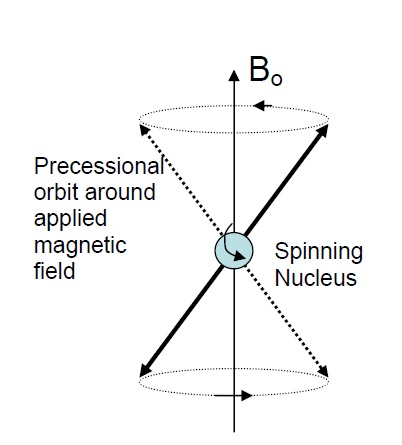
\includegraphics[width=.375\textwidth]{figures/aBackground/nucleus_precess}  
	\caption{The figure illustrates how the nucleus precess and spin in relation to the applied magnetic field $B_0$ surrounding it. The vectors, indicating the precessing, can go opposite or along the magnetic field depending on the nucleus energy state. \cite{Edwards}}
	\label{fig:back:nucleus_precess} 
\end{figure}  
A radio frequency pulse (RF pulse) tuned to the precession of the nuclei is transmitted in the vicinity of the nuclei. The RF pulse is absorbed by the nuclei and more, favorably half of the targeted nuclei population, will enter the high energy state, leaving the longitudinal magnetization to equal zero. The number of nuclei that flip is determined by the amount of energy the RF pulse injects, and the nuclei only exchange energy efficiently if the frequency of the energy from the RF pulse matches the precession rate. The RF pulse furthermore shifts the precession of the nuclei into same phase angle, which creates resonance, and a net magnetization pointing 90$^\circ$ to the longitudinal magnetization. This magnetization is called the transverse magnetization. The coherent nuclei produce a radio signal, or free induction decay signal (FID signal), that can be detected by a radio antenna. 
After the RF pulse is removed, the nuclei will relax into baseline state. Firstly, the spins of the nuclei will repel each other, as they are positively charged, and thus shift phase. The net magnetization will return to zero. This relaxation is called $T_2$ or “spin-spin” relaxation, as the energy exchange between the nucleus spins is causing the relaxation. A second relaxation appears as the high energy nuclei returns to the low energy state. The energy that was previously absorbed by the nuclei is dissipated in to the surrounding lattice in the form of heat. During this relaxation the longitudinal magnetization is regrown. This relaxation is called $T_1$ or “spin-lattice” relaxation, as the spins transfer energy to the surrounding lattice. \cite{Bharath2008}
{\Large (Insert illustration)} \\
The hydrogen nuclei are located in different local environments in the body. Some are for instance associated with free-floating water molecules, while others are associated with structural and storage molecules such as proteins and lipids, and thus more fixed in position. The nuclei have different $T_1$ and $T_2$ relaxation characteristics, depending on the local environment or tissue they are associated with. This can be accentuated and measured in NMR. \cite{Bharath2008} \\
The chosen pulse sequence is key to how the tissue will be portrayed in an image, and is described by the $T_{echo}$, time before the FID signal is measured, and $T_{rep}$, time before a new RF pulse is applied. In a case of nuclei associated with lipids and water molecules, the nuclei in lipids are fixed and will have a fast $T_1$ relaxation after exposure to a RF pulse . Meanwhile the nuclei in the water molecules will maintain being in a synchronized phase. At $T_{echo}$, the nuclei associated with the lipids will have a low amplitude FID signal, as the transverse magnetization is weak, and the nuclei associated with the water molecules will have a high amplitude FID signal, as the transverse magnetization is strong. The water molecules will be assigned a white color on a greyscale image and the lipids as dark grey/black. In this case there is a long $T_{echo}$ and a long $T_{rep}$, and is referred to as $T_2$-weighted MRI. \cite{Bharath2008} \\
In case of $T_1$-weighted MRI, the $T_{echo}$ and $T_{rep}$ are short. As in $T_2$-weighted MRI a RF pulse is applied and the nuclei associated with lipids will quickly return to baseline state and the water molecule nuclei will remain a strong transverse magnetization. At this time point a second RF pulse will be induced, referring to the short $T_{rep}$. Now the lipid nuclei will return to a strong transverse magnetization state and excite a high FID signal. More low energy state nuclei of the water molecules will absorb the RF pulse and shift to a high energy state, leaving a majority of nuclei in a high energy state. The water molecule nuclei now has a weak transverse magnetization and 180 degrees longitudinal magnetization, thus producing a low-amplitude FID signal. A short $T_{echo}$ after the second RF pulse then shows lipids as white and the water molecules as dark grey/black in a greyscale image. \cite{Bharath2008} 


\section{Functional MRI}

Many different techniques exist to accentuate different tissues, physiological phenomena etc. using MRI, of which a few will be described further in the following section. 

\subsection{Introduction to BOLD fMRI}
Functional magnetic resonance imaging measure the metabolic changes associated with different neurological tasks in different brain areas. fMRI offers advantages predominantly, high temporal and spatial resolution, low cost, and most importantly being non-invasive, which has made it a exceedingly popular method for imaging brain activity. The versatility of fMRI has made it very important tool in being a biomarker for diseases and to study the efficacy of pharmaceuticals. The method offers high resolution of anatomical structures and localization and visualization of vessels. \cite{Glover2011} 

Multiple steps in forming and transmitting a neurological signal requires energy Adenosine tripolyphosphate (ATP) consumption e.g. reception and reformation of an action potential. When activating a brain area as done in the most often used example, finger tapping, the ATP starts to be processed, leading to a decrease in oxygen concentration and increase in waste. Thereby the metabolic need for oxygen increases. As the movement is planned and executed, factors, which are present in the local tissue of the corresponding brain area, activate a vasodilation, increasing the blood flow to that area and reestablishing the local homeostasis. Though one special and not fully understood phenomenon occurs during this process. More oxygenated blood than needed to compensate for the offset is delivered. Thereby an overshoot occurs. The increase in neural activity in that specific area thereby permits two conditions which can be assessed through fMRI, being the cerebral blood flow and blood oxygen level dependent contrast. An example illustrating the measurable hemodynamic response can se found in \figref{fig:back:stim}\cite{Glover2011,Poldrack2011}

\begin{figure}[H]                 
	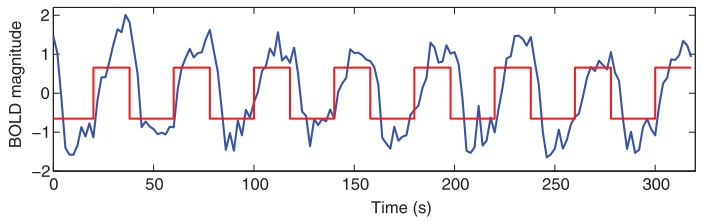
\includegraphics[width=.69\textwidth]{figures/aBackground/stimuli_vs_response}  
	\caption{Figure showing an induced series of stimuli (red) and the hemodynamic response to the neural activity measured using BOLD (blue). It is shown that the measurable hemodynamic response is delayed compared to the stimuli. \cite{Poldrack2011}}
	\label{fig:back:stim} 
\end{figure}


As established in the above section the BOLD signal is effected by the neural activity producing changes in the local blood flow, blood volume and blood oxygenation. The crucial part to why MRI can detect this natural contrast, is that fully oxygenated blood, is diamagnetic and fully deoxygenated blood has four unpaired electrons thereby making it highly paramagnetic. Thereby more oxygenated blood in the area the larger the contrast, compared to other brain regions, is seen as illustrated in \figref{fig:back:bold}. \cite{Glover2011,Khanna2015,Poldrack2011}

\begin{figure}[H]                 
	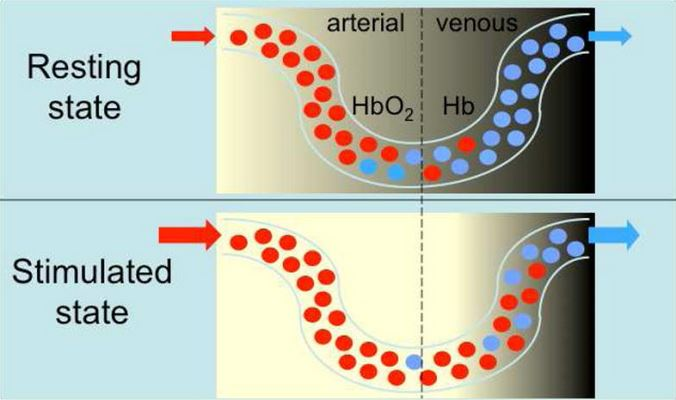
\includegraphics[width=.52\textwidth]{figures/aBackground/bold_response}  
	\caption{Illustration of how the difference in oxygen concentration in the hemoglobin change the magnetic properties, resulting in a higher measurable contrast \cite{Glover2011}.}
	\label{fig:back:bold} 
\end{figure}

This change in local magnetic properties increases the magnetic susceptibility leading to a greater MRI signal when acquiring an $T_2^*$- weighted sequence.  

\section{MR image reconstruction}

Different pulse sequences and certain physiological properties that can be exploited with certain pulse sequences, have been laid out in the previous sections. This section aims to describe how the corresponding echo signals are reconstructed as a MR image.

Following the Lamour frequency \eqref{eq:lamour}, the main magnetic field causes all hydrogen nuclei to precess with the same frequency. Without any specification of spatial localization a MRI of a human body would consist of a single number. To prevent this, separate coils in the x, y and z directions are introduced. These coils can be adjusted in position, and thus produce gradient magnetic fields with a varying strength depending on position. According to the Lamour frequency the nuclei will precess with different frequencies when in a magnetic field with varying strength. The gradients can be turned on in combination to create any direction in space. These varying frequencies can be exploited to separate parts of the anatomy and ultimately illustrate a desired area. As mentioned, the nuclei only exchange energy efficiently if the frequency of energy, or RF pulse, matches the precession rate. Thus, by altering the magnetic field along the body in one direction, z-direction for the sake of the example, the nuclei will have slightly different precession rates, and the RF pulse will only efficiently affect a desired slice of the nuclei.
The nuclei of that slice now precess at the same rate. To get an image with a spatial resolution, the voxels that make out the image needs to be discriminated between. By turning on the gradient of the x-direction the lines in the y-direction are now encoded with a particular frequency. This gradient functions as a frequency encoding gradient, and is illustrated in \figref{fig:back:gradient}. \cite{Bharath2008} \\
 \begin{figure}[H]                 
	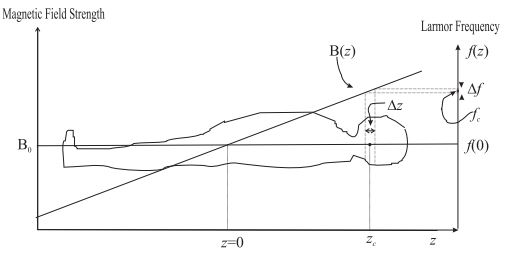
\includegraphics[width=.7\textwidth]{figures/aBackground/gradient}  
	\caption{The position of the slice is specified through the direction of the frequency encoding gradient ($B(z)$) and though the central frequency of the emitted RF pulse ($f_c$). The thickness of the slice is dependent on the steepness slope of $B(z)$, and on the bandwith of the emitted RF pulse $(\delta f)$. \cite{Bharath2008}}
	\label{fig:back:gradient} 
\end{figure}
Turning the y-gradient on and quickly off, will de-phase the nuclei while still remaining the same frequency as before. This gradient functions as a phase encoding gradient. When comparing two locations approximately one voxel apart in the x-direction, then based on the amount of gradient strength difference, there will be a certain amount of change in phase between the spins spread across that distance. The farther away from isocenter, where the magnetic field strength is $B_0$, the higher the change in phase will be. This notion is used to assign the correct spatial location of each voxel, when reconstructing the FID signals into an image. This phase encoding procedure is done in different gradient strengths in iterations to assign unique phases to the nuclei in the both directions. One iteration of a certain strength of the phase encoding gradient followed by a measurement is performed at a time. The only change per iteration is the phase encoding gradient strength. These iterations are then series of measurements acquired at different points in time, where each entry of the slice then represent a certain signal intensity. This time domain measurement is referred to at the raw data. \cite{Bharath2008}\\
The next step is to Fourier Transform (FT) the raw data, which will yield frequency information to the acquired signal intensities. This step gives a summation of the signal intensities at the different frequencies produced by the frequency encoding gradient. This is called the k-space, as the k-numbers of a signal describes its relative orientation and frequency. The k-space image contains the contrast in the center and the resolution in the periphery, as there is low or no phase encoding at the center and increasing towards the periphery, giving more brightness in the center and dimmer tones in the periphery. To allocate the voxels in correct spatial localization an inverse 2D discrete FT is performed on the k-space image. This provides the desired image of the anatomy slice. \cite{Bharath2008} \Figref{fig:back:kspace} shows the acquired signal in k-space and the reconstructed image after the Fourier Transform. 

\begin{figure}[H]                 
	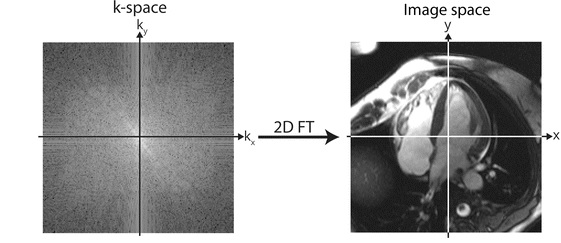
\includegraphics[width=.8\textwidth]{figures/aBackground/k_space}  
	\caption{A depiction of the acquired signal represented in k-space and the resulting reconstructed image after the inverse 2D Fourier Transform \cite{Syed2015}.}
	\label{fig:back:kspace} 
\end{figure}
\section{Stimuli Design} \label{sec:Stim}

The following section will describe different standards of designing experiments where the impact of a given stimuli is used to assess the subsequent brain activation. The impact of stimuli on the hemodynamic response and how it is transformed into the hemodynamic response function (HRF) used analysis will be further explained, adding to the knowledge gained in \secref{sec:fMRI}.

In order to accomplish a well designed experiment, the researcher must consider the multiple types of stimuli delivered, including the form and duration of these. The researcher must be aware of the timing of events in the scanning session and any responses provoked. Additionally, the researcher should have general knowledge of where in the brain activation is seen and how the hemodynamic response will be presented. \cite{Moayedi2018} 

Doing cognitive experiments using fMRI, two main design types are utilized, by either using a block- or event-related design.   
Event-related design is inducing a series of very short lasting stimuli used to investigate single hemodynamic response. A characteristic of this method is that it permits the possibility of increasing and decreasing the interval between stimuli. Thereby the theoretical likelihood of subject confounds should be reduced as the interval would not become predictable. Event-related stimuli design further allows more temporals characteristics to be inspected, compared to a block design. Characteristics could be hemodynamic response in duration and amplitude. \cite{Chee2003}  \\
Block design works by performing a series of less but longer stimuli. Block designs are ideal for experiments involving detection of small differences in BOLD signal across various test conditions where its statistical power is superior. Furthermore, if there is artifacts present they are more easily detected in the signal time course, because of the signals temporal structure. A block design is easier to design than an event-related, as randomization of intervals of stimuli is not required. The design instead focuses on the total number of stimuli used, block length, inter stimulus interval, block length and TR. An illustration of both design types can be found in \figref{fig:back:e_vs_b}. \cite{Chee2003}       

To enable use of the hemodynamic response in fMRI analysis, it needs to be transformed in order to represent the ideal physiologic response to the stimulus. Thus, portraying the biological delay from stimuli to response. Therefore stimulus in the design is combined with the hemodynamic response function through convolution. Thus making a function that models how the BOLD signal would be represented if the voxel activity increased in a given area each time stimuli is induced. \cite{Moayedi2018}

\begin{figure}[H]                 
	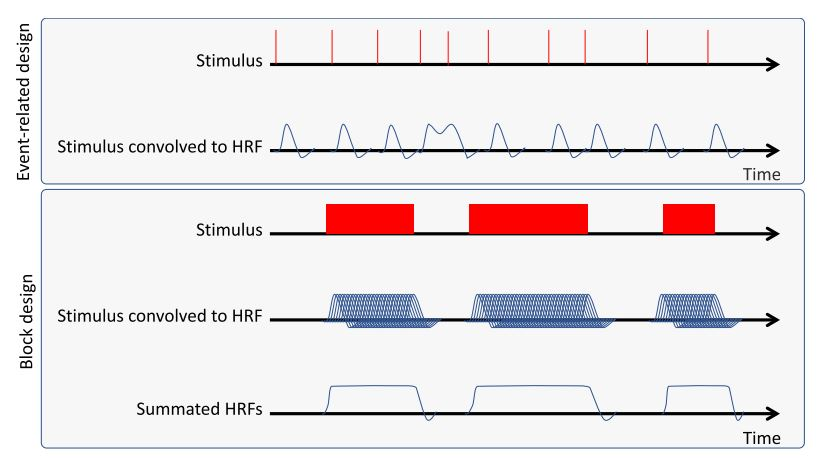
\includegraphics[width=.8\textwidth]{figures/aBackground/event_vs_block}  
	\caption{The top image show the event-related stimuli design and the stimulus convolved with the hemodynamic response function. The lower image depicts a block design, the stimulus convolved with hemodynamic response function and the summated HRF response.  \cite{Moayedi2018}}
	\label{fig:back:e_vs_b} 
\end{figure}

 


\section{Standard MRI pre-processing}
There are multiple ways to preprocess fMRI images, some depending on the apparent application. However, there is a standard set of methods that is mostly usually used across all applications. The following section seek to elucidate some of the most commonly used correction methods including the ones considered for the standard preprocessing method used in this project. 

\subsection{Techniques for quality control}
Conducting a continues appropriate quality control is highly recommended to do across all applications, as the example on \figref page 35 shows. Various scanner artifacts can occur while acquiring an MRI series. Spike artifacts are seen as a regular pattern of change in brightness across the entire image. This problem can occur due to instability inside the scanner derivering e.g. from electrical discharges.  
The artifact called ghosting can occur mainly due to two reasons. One being an offset in phase between different lines in K-space and the other due to periodic motion as in heartbeat and respiration. Ghosting can be seen as light copies of the object appearing to either side of the object. Both types of artifacts can corrupt the information contained in the images. However, artifacts of this kind rarely present themselves in newer scanners, nevertheless it is still recommended to control the quality of the scan. \cite{Handbook}

\subsection{Distortion correction}

Some fMRI acquisition methods, including the most widely used method of gradient-echo echo planar imaging, suffers from artifacts at regions air and tissue meet. This could be the areas of ear canal and sinuses. Inhomogeneity in the magnetic field in these areas can cause two types of artifacts, dropout and geometric distortion. A dropout will result in a reduced signal intensity in region close to the air to tissue passage. When a dropout during an acquisition occurs the lost signal cannot be restored and the damage is permanent. Therefore it is wise to consider the appropriate acquisition method taking the area of interest into addition. Air to tissue passages can also be subject to spatial distortion due to inhomogeneity created in the magnetic field. This will lead to structures not being located correctly in the captured image. This distortion makes is difficult to align two different scan, as done when aligning fMRI images with structural images. 
The spatial distortion can partially be corrected by employing field maps. In order to do a field map, the pulse sequences from the scan are needed. The process involved acquiring images at two different echo times. This result in images with two different phases which can be used to compute the field inhomogeneity. Thereby it becomes possible to calculate the relative distance each voxel has shifted. This makes up a map for the distance shift for each voxel, and by inverting the map the original image can be restored.  

\subsection{Slice timing correction}

Acquiring fMRI scans is nearly always done in two-dimensions, where the slices are taken one by one. This can either be in an ascending, descending or interleaved order. Interleaved order \fxnote{think it is done to avoid crosstalk} is sequentially skipping every either odd or even slice and then afterwards do to skipped slices. Regardless of which order the slices are acquired, a difference in effect in each slice to the same hemodynamic response will be present due to the time difference in the slices. The difference in time between slices can range up to a couple of seconds depending on the acquisition protocol. 
The difference in slice timing constitutes a problem when analyzing the data. The data is formed into statistical model, but since this model assumes that all slices are acquired at the same time point, the actual signal and the model creates a mismatch. To counter this problem slice timing correction was introduced. The common approach in this method is to choose a reference slice, usually the slice acquired at T/2, and use this slice to interpolate the others. Linear interpolation can be used for simplicity, but most often sinc interpolation is used as it imposes less smoothing to the signal. 

\subsection{Motion correction}

Having to deal with motion artifacts when doing MRI is inevitable, since even the best subjects will not be able to hold still. Even subtle movements as swallowing will be visible in the raw acquired image. 

Multiple internal and external factors can cause a subject to move. Internal factors are physiologic motion. The heartbeat causes a pulsating movement which makes the brain move. Additionally motion created during respiration can cause small changes in the magnetic field around the head. External factors like imposed stimulus might cause the subject to make sudden movements. Often when doing fMRI the brain activation is measured while the subject is subjected to some kind stimulus. The stimulus would make the patient move, while the brain center would be active, therefore it is easy to mistake brain activation with stimulus correlated movement when analysing the data, resulting in a weaker/false statistical analysis. 

Motion during image acquisition can result in two primary effects, being Bulk motion and Spin history. Bulk motion refers to the movement of the head as a whole and requires standard correction methods, e.g. the images throughout the series to be realigned to a reference image. The effect of Bulk motion can be visual in the entire image of the brain, but the effect will be most predominant at the edges of the brain. Here the artifact will be noticeable as either a drop or increase in intensity as a voxel would switch from containing brain tissue to suddenly not, during head motion.  
Spin history is associated head movement interfering with MRI signal. The interference occur during acquisition when a voxel of excited protons are moved in to a neighbouring slice. The scanner will thereby receive a different signal than expected which is not correctly represent the actual tissue properties. This results in an image where the intensities change in a striped pattern, visible when acquiring slices in interleaved order. The standard motion correction methods cannot cope with this type of artifact, but Independent Component Analysis (ICA) might be to correct for this artifact. 

Motion correction techniques on monday 

\subsection{Spatial smoothing}



\section{Independent Componant Analysis}
ICA has proven to be a very successful tool in separating noise from wanted signal in BOLD-signals, making it a very desireable tool in fMRI.\cite{Salimi-Khorshidi2014} 


\section{Principal Component Analysis}

Principal Component Analysis (PCA) is a well renowned and widely used analysis tool, capable of finding the most defining variables in a dataset. This facilitates finding the components that are the most saying for the dataset and makes it possible introduce dimensionality reduction, lowering the amount of redundant information. The PCA is used to transform a set possibly correlated variables into a set of uncorrelated components, called principle components. Each principal component (PC) is
orthogonal on the former and are uncorrelated and have zero covariance. They each define the largest
variance in an axis, such that PC 1 describes the direction of the maximum variance of the dataset. Each
following PC describes the next highest variance of the dataset, with the constraint that is orthogonal
and has zero covariance with any of the former PCs. PCA is the orthogonal projection of data onto a
lower dimension linear space.  A PC is found by minimizing the variance by projecting the feature values (blue dots) onto the line (now red dots) describing the highest variance in the data set (black line) as seen on \figref{projection}. The PC is found by minimizing the mean square distance between the data points. \cite{Jolliffe1986}

\begin{figure}[H] 
	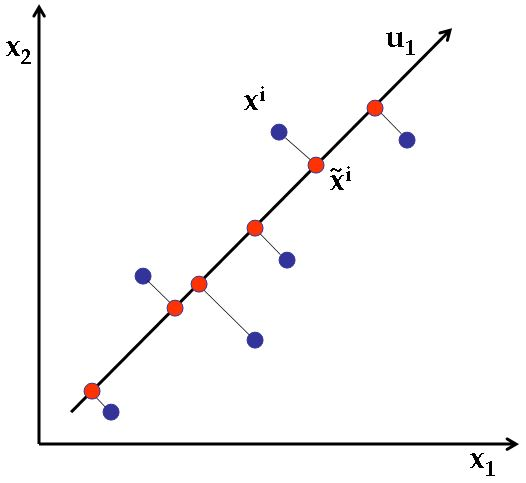
\includegraphics[width=0.38\textwidth]{figures/aBackground/projection}
	\caption{Two-dimensional example of projection of data variables (blue dots) onto PC axes (black). $(u_1)$ indicates the direction of the eigenvector. \cite{PCA2018}}
	\label{projection}
\end{figure}

The algebraic method of calculating the PCs can be done by using Singular Value Decomposition (SVD). The first step is to compute the squared cross product matrix of variances and covariances among every pair of the variables in the data set, where the diagonals are the variances and the off-diagonals are the covariances, as done in the following equation:
%\vspace{-20pt}
\begin{equation}
S = X \textquoteright X
\end{equation}
Where S is the cross product and X is the dataset matrix. When finding the PCs it includes an eigen-analysis of S. The eigenvalues of are solutions to the following equation:
%\verticalspace{1}
\begin{equation}
| S - \lambda I |  = 0
\end{equation}
Where $\lambda$ is the variances of each PC and I is the identity matrix. After solving for $\lambda$ the eigenvectors can be solved through the following equation:
\begin{equation}
det | S - \lambda I | b_{i} = 0
\end{equation}
Where $b_{i}$ is used to calculate the eigenvectors as in:
\begin{eqnarray}
u_{i} = \frac{b_{i}}{\sqrt{b_{i}^{\textquoteright} b_{i}}}
\end{eqnarray}
Where $u_{i}$ is the i number of eigenvectors that contain a contribution to the principal components.
The SVD orders the eigenvalues by size $\lambda_{1} > \lambda_{2} … > \lambda_{i}$. The scores for each PC is equal to the corresponding eigenvalue for that exact axis. The eigenvalues describe how much of the variance is accounted for by the associated PC. Summation of all eigenvalues accounts for the total variance of the data set; this is called the trace. To find how much the each PC accounts for, the eigenvalue of that PC is divided by the total variance: $\%~ of~ total~ variance~ = \frac{\lambda_{i}}{Trace}$. This can be used for deciding how many components are significant and by how much the dataset can be reduced. \cite{Jolliffe1986}



\section{General Linear Model}

In order to determine if a task or stimuli has made a significant contribution to the measured BOLD signal, each voxel in the scan needs to be evaluated. The following section will introduce the general linear model (GLM) as it is the most used tool for fMRI analysis during the past 20 years \cite{Poline2012}. 

The GLM is a well considered and used analysis tool constituting a simple way of doing standard statistical analysis on fMRI. The overall goal of the GLM model is to determine how well the time course of the scan corresponds to the known used experimental interference.  In an fMRI case that means, how well the BOLD signal over time fits the time course of the predicted signal given by the imposed stimuli, causing brain activity. This statistical test is carried out for each voxel independently of its neighbor across the scan resulting in thousands of statistical test in one scan. \cite{Moayedi2018,Monti2011} To explain the implementation of a GLM we can use the example presented by \textit{Monti et al.} An acquired BOLD signal will throughout a time series, of \textit{n} images, have a varying output signal. The signal in a voxel $Y$, at any time point, can be seen as a summation of predictor variables (stimuli regressors) $X$,  additional nuisance regressors modeling noise $X$, a scaling parameter for each regressor $\beta$, and an error term $\epsilon$. This can be presented in the GLM's basic from as \cite{Monti2011}: 
\begin{equation}
Y=X\beta+\epsilon
\end{equation}

Expanding this formulation into a complete scan, including multiple regressors, can be presented on a matrix form. A depiction of a GLM design matrix incorporating the factors making up the BOLD signal can be seen in \figref{fig:GLM}. 

\begin{figure}[H] 
	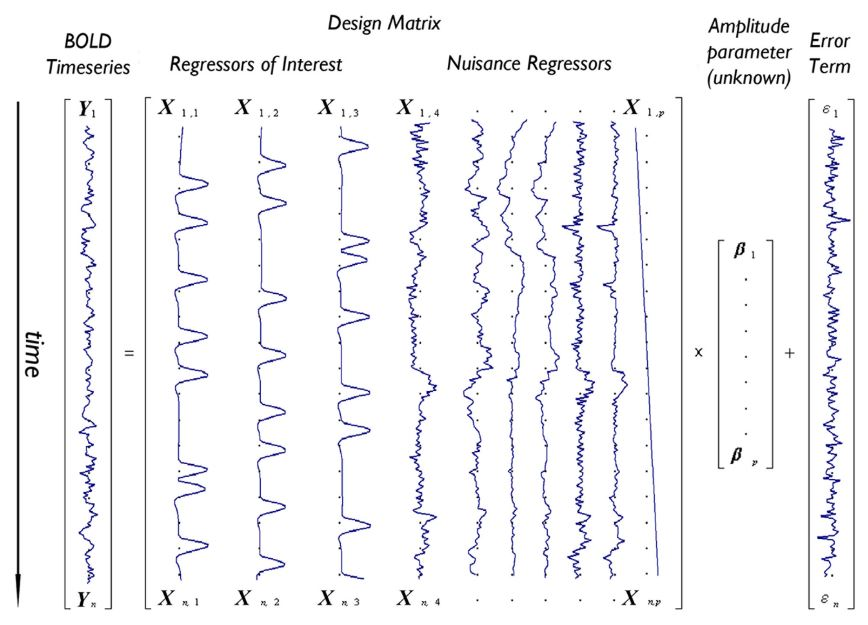
\includegraphics[width=0.90\textwidth]{figures/aBackground/GLM}
	\caption{Illustration of a design matrix for a given GLM model, describing the BOLD time series $Y_n$, the regressors of interest $X_{1,1}, X_{1,2}, X_{1,3}$, the additional nuisance regressors $X_{4..p}$, the amplitude parameter $\beta_{1..p}$ and the error terms $\epsilon_{1..n}$. \cite{Monti2011}}
	\label{fig:GLM}
\end{figure}



The predictor variables are found by modeling what is known or predicted as output. The predictors of interest would come from hemodynamic response curve convoluted with stimuli design as presented in \secref{sec:Stim}. GLM models will often introduce nuisance predictors as well used to model variables such low frequency drift and motion to make a more robust model. These are non interest regressors, as they do not resemble the wanted signal, being the stimuli induced. The amplitude parameter is the unknown weight scaling the magnitude between each predictor value and the data. They describe the strength of the relationship between that regressor and the voxel's BOLD signal course of activation. The error term contains the value for each observation, which can not be explained by the wighted sum of the amplitude parameter. \cite{Moayedi2018,Monti2011} 

The goal is to estimate the value of the scaling parameter $\beta$ for all regressors and afterwards determine if any regressor significantly account for the variance found in the BOLD signal. A regressor associated with the measured BOLD signal should hypothetically show a greater value for the voxels in the brain area corresponding to a given task. E.g. finger tapping would show greater $\beta$ values in the motor cortex. Methods of estimating $\beta$ values for regressors are ordinary least squares (OLS), generalized least squares (GLS) and the smoothing and sandwich method. The OLS methods estimates $\beta$ by minimizing the sum of squared residuals \cite{Monti2011}: 

\begin{equation}
\sum_{i=1}^{n}(Y_i-X_i\times\hat{\beta})^2
\end{equation}  

, where Y is the observed signal, X is the predicted signal which is scaled by $\beta$. $\beta$ and the variance of $\beta$ can be estimated by: 

\begin{equation}
\hat{\beta}=(X^TX)^{-1}X^TY
\end{equation}

\begin{equation}
var(\hat{\beta})=\sigma^2(X^TX)^{-1}
\end{equation}

The application of this method rest on the following assumptions being fulfilled: Error terms are independently and Gaussian distributed with zero mean, the regressors in the matrix are independent of error and non stochastic and known and no regressor is a linear transformation of another regressor. \cite{Monti2011}    






\chapter{Methods}


\section{FSL FIX}

The following section will describe the implementation of FIX, which introduces a faster and more standardized approach to ICA-based noise cleanup \cite{Salimi-Khorshidi2014}. The FIX method is a more extensive approach, which adds another layer of preprocessing to the standard preprocessing. This meant that before initiating FIX the data needed to undergo the exact same steps as in the standard preprocessing presented in \secref{sec:std}. Following the standard preprocessing, the functional scan underwent an ICA to split the sources in the acquired signal, which ideally would separate signal of interest from noise. Afterwards an analysis of optimal number components in which the data should be split was performed. The FIX tool uses a classifier to separate noise components from signal components. The classifier needed to be trained before it applied on a new data set. In \figref{fig:meth:fix} a flowchart showing the steps for both the training data set and the test data set in the FIX pipeline is illustrated. 


\begin{figure}[H]                 
	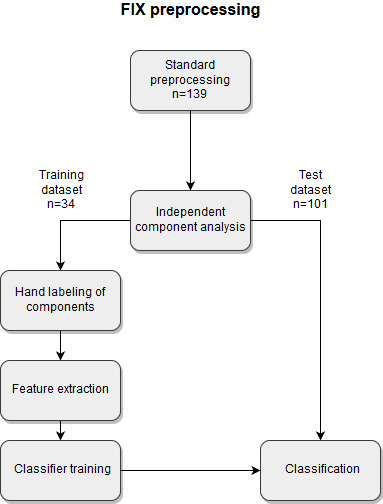
\includegraphics[width=.6\textwidth]{figures/bMethods/FIX_flow} 
	\caption{Flowchart illustrating the two datasets and the corresponding steps that was applied to each dataset in the FIX pipeline. Initially, MELODIC was used to estimate independent components. These components were subsequently hand labeled, and used to train the classifier along with 186 features extracted from each component. The trained classifier could then be used to identify the the source of each component from a test data set.}
	\label{fig:meth:fix} 
\end{figure}

%
%
%\subsection{Calculation of Independent Components}
%
% For a single session ICA the MELODIC FSL program utilizes the FastICA algorithm to obtain independent components. This section seeks to lay out how the FastICA algorithm works and which mathematical techniques that are exploited. \\
% As stated in \secref{sec:ICA}, from the central limit theorem we get that observed mixed signals tend to have a more Gaussian distribution than the individual source signals, since the observed signal is a summation of the source signals. As a result of this, an approach is to find a linear transformation that leaves the source signals as non-Gaussian as possible. This principle is what the FastICA algorithm is build up around. \\
% Firstly the vector \textbf{b} is introduced, which is a row vector in the mixing matrix \textbf{A}, and is used in a linear combination:
% 
% \begin{equation}
% y = \mathbf{b^T}\mathbf{x}
% \end{equation}
% 
% By substituting $\mathbf{x} = \mathbf{A}\mathbf{s}$ in the previous equation:
% 
% \begin{equation}
% y = \mathbf{b^T}\mathbf{A}\mathbf{s} = \mathbf{q^T}\mathbf{s}
% \end{equation}
% 
% Where $\mathbf{q^T} = \mathbf{b^T}\mathbf{A}$. From this it can be deduced that \textit{y} is an IC, when only one of the entries of \textbf{q} is non-zero and the rest is zero. This means that there is no addition of any random processes and the component will be as non-Gaussian as possible. An IC can then be obtained by calculating a value of \textbf{b} that maximizes the non-Gaussianity of the distribution of $\mathbf{b^T}\mathbf{x}$ as $\mathbf{b^T}\mathbf{x} = \mathbf{q^T}\mathbf{s}$. This gives an optimization problem with convergence at local maxima. As there exist a local maximum of the non-Gaussianity for both \textit{s} and ${s_i}$, the optimization landscape in a n-dimensional signal gives a total of \textit{2n} local maxima.
% To be able to optimize according to non-Gaussianity, a quantitative measure of such is needed. This can be provided by the fourth order cumulant, kurtosis, which is zero when \textit{y} is Gaussian distributed and non-zero when \textit{y} is non-Gaussian distributed (negative when sub-Gaussian and positive when super-Gaussian). Given this property and the central limit theorem, the linear combination $\mathbf{b^T}\mathbf{x}$ that yields an IC can be found at the local maxima of the absolute value of the kurtosis of \textit{y}. The kurtosis of \textit{y} is given by:
% 		
%\begin{equation}
%kurt(y) = E{y^4} - 3E{y^2}^2
%\end{equation}
% 		
%As the whitening of the data results in unit-variance, \textit{kurt(y)} can be modified to:
%		
%\begin{equation}
%kurt(y) = E{y^4} - 3
%\end{equation}
% 		
%To simplify the theoretical analysis furthermore the linear properties of kurtosis for sums of variables can be utilized. For two random variables, \textit{$x_1$} and \textit{$x_2$}, it holds that:
%
%\begin{equation}
%\begin{split}
%kurt(x_1 + x_2) &= kurt(x_1) + kurt(x_2) \\
%kurt(\alpha x_1) &= \alpha^4 kurt(x_1)
%\end{split}
%\end{equation} 			
%For the multiplicative scalar textit{$\alpha$} the kurtosis is non-linear, and the optimization problem can thus be written as:
% 			
%\begin{equation}
%kurt(y) = \sum_{i} q_{i}^{4}kurt(s_i)
%\end{equation}
% 			
%Due to the whitening of the data, where \textit{y} has unit-variance, a constraint is put on the vector \textbf{q}. Since $E{y^2} = \sum_{i}^{n} q_{i}^{4}$ the vector \textbf{q} is constrained to the unit-sphere. For the whitened data \textbf{z} a linear combination $\mathbf{w^T}\mathbf{z}$ that maximizes non-Gaussianity is sought for. From the fact that $\mathbf{q} = \mathbf{V}\mathbf{A})^{T}\mathbf{w}$, the following is given:
% 			
%\begin{equation}
%\parallel \mathbf{q} \parallel^{2}= (\mathbf{w}^{T}\mathbf{V}\mathbf{A})(\mathbf{A}^{T}\mathbf{V}^{T}\mathbf{w}) = \parallel \mathbf{w} \parallel^{2}
%\end{equation}
% 			
%This expresses that constraining the vector \textbf{q} to lie on the unit sphere equally constraints \textbf{w} to the unit sphere. The objective is now to find a value of \textbf{w} that maximizes the absolute value of the kurtosis of $\mathbf{w^T}\mathbf{z}$. Whitening further allows the linear combination $\mathbf{w^T}\mathbf{z}$ to be understood as projections on the line in a 1-D subspace spanned by \textbf{w}. What is sought for is the direction of \textbf{w} where the absolute value is maximized, which then makes out an IC. \\
%To solve this optimization problem a commonly used technique is the gradient algorithm to reach convergence at local maxima, thus calculating the direction where the absolute value of the kurtosis of $\mathbf{w^T}\mathbf{z}$ is growing most strongly. The can be computed as the following:
% 			
%\begin{equation}
%\frac{\delta|kurt(\mathbf{w^T}\mathbf{x})|}{\mathbf\delta\varTheta{w}} = 4 ~ sign ~ (kurt(\mathbf{w^T}\mathbf{z})[E{\mathbf{z}(\mathbf{w^T}\mathbf{z})^{3}} - 3\mathbf{w}\parallel\mathbf{z}\parallel ^{2}]
%\end{equation}
% 				
%However, there is in practice disadvantages associated with using the gradient algorithm, e.g. slow convergence rate and is dependent on a proper choice of learning rate. The fixed point algorithms is suggested as a faster algorithm alternative. At the stable point of the gradient algorithm, the gradient is pointing the direction of \textbf{w}. It is only in this case that \textbf{w} will not change direction when adding the gradient. This notion about the gradient of the absolute value of the kurtosis can be used to form a fast fixed point algorithm, or the FastICA algorithm:
% 				
%\begin{enumerate}
%\item $\mathbf{w}  \leftarrow  E\{{\mathbf{z}(\mathbf{w^{T}\mathbf{z})^3}}\} - 3\mathbf{w}$
%\item $\mathbf{w}  \leftarrow \mathbf{w} / \parallel \mathbf{w} \parallel$
%\end{enumerate}
% 									
% 					
%The right hand side is firstly computed and assigned to \textbf{w}, which afterwards is normalized to follow the constraint of $\parallel \mathbf{w} \parallel ^2 = 1$. By iterating over this convergence is reached at an ultimate \textbf{w}, where $\mathbf{w^{T}\mathbf{z}}$ is an IC. In order to obtain several IC’s the process is repeated, with the constraint that \textbf{w} must be orthogonal to all previously computed \textbf{w}. 
% 						



	
\urlstyle{same}
\printbibliography
\clearpage



\cleardoublepage
% BILAG
%\begin{appendices}
%	\chapter{Appendices}
%
%\end{appendices}


\end{document}
